% !TEX root = paper.tex
% !TEX program = pdflatex + bibtex
\documentclass[conference]{IEEEtran}
\IEEEoverridecommandlockouts

\usepackage{cite}
\usepackage{amsmath,amssymb,amsfonts}
\usepackage{algorithmic}
\usepackage{graphicx}
\usepackage{textcomp}
\usepackage{xcolor}
\usepackage{listings}
\usepackage{booktabs}
\usepackage{multirow}
\usepackage{url}
\usepackage{hyperref}
\usepackage{subcaption}
\usepackage{float}
\usepackage{titlesec}

\titleformat{\section}{\normalfont\Large\centering}{\thesection}{1em}{}

% CUDA listing style
\lstdefinestyle{cuda}{
  language=C++,
  basicstyle=\ttfamily\scriptsize,
  keywordstyle=\color{blue}\bfseries,
  commentstyle=\color{green!50!black}\itshape,
  stringstyle=\color{red!70!black},
  numbers=left,
  numberstyle=\tiny\color{gray},
  numbersep=5pt,
  frame=single,
  breaklines=true,
  captionpos=b,
  morekeywords={__global__,__device__,__shared__,__constant__,
                __syncthreads,__syncwarp,atomicAdd,__ldg,
                __launch_bounds__,blockIdx,blockDim,threadIdx,
                gridDim,float3,int3,uint32_t,cudaStream_t},
  tabsize=2
}
\lstset{style=cuda}

\def\BibTeX{{\rm B\kern-.05em{\sc i\kern-.025em b}\kern-.08em
    T\kern-.1667em\lower.7ex\hbox{E}\kern-.125emX}}

\begin{document}

\title{GPU-Accelerated Discrete Element Method (DEM) Simulation of a Snowball Avalanche Dynamics on NVIDIA Maxwell}

\author{
\IEEEauthorblockN{Maurizio Grisotto}
\IEEEauthorblockA{\textit{Politecnico di Torino}\\
Turin, Italy 2026\\
s336145@studenti.polito.it}
}

\maketitle

\begin{abstract}
We present a real-time simulation of a growing snowball rolling down an inclined slope, capturing static snowpack particles via a Discrete Element Method (DEM)-inspired contact adhesion model as a potential component of a real-time game graphics engine.
This paper investigates the concepts covered in the “GPU Programming” course through the implementation of a snowball simulation with 3 different applications: CPU Naïve, CPU-Optimized, and GPU.
Both the algorithmic/performance aspects and dynamic Vulkan rendering (GPU version only) were addressed.
A theoretical analysis of the multi-GPU extension scenario is also provided.
The simulation is implemented entirely in CUDA targeting NVIDIA Maxwell GPUs (SM~5.0/5.3) and features a multi-stream pipeline with adaptive kernel fusion, warp-cooperative, shared-memory tiling, lock-free atomic capture, spatial hashing with CUB radix sort, and zero-spill register allocation across all kernels.
We detail each optimization with quantitative analysis of occupancy, memory bandwidth, and launch overhead trade-offs.
The GPU implementation is benchmarked against scalar (SISD) and SSE/NEON~+~OpenMP (SIMD) CPU baselines on a laptop GTX~960M and a Jetson~Nano, demonstrating the effectiveness of architecture-aware CUDA programming on resource-constrained Maxwell hardware.
\end{abstract}

\begin{IEEEkeywords}
CUDA, GPU programming, Discrete Element Method, particle simulation, Maxwell architecture, shared memory tiling, spatial hashing, kernel fusion, occupancy tuning
\end{IEEEkeywords}

% !TEX root = ../paper.tex
\section{Introduction}
\label{sec:introduction}

Granular-material simulations are central to computational physics and
engineering, with applications ranging from geotechnical hazard prediction to
visual effects in games and films. The \emph{Discrete Element Method}
(DEM)~\cite{cundall1979} models granular media as collections of individual
particles interacting through pairwise contact forces, providing a physically
faithful representation of phenomena such as avalanches, landslides, and
snowfall accumulation. However, DEM simulations are computationally demanding:
at each timestep every particle must detect contacts with its neighbours and
resolve penalty-based forces, yielding an $O(N \cdot k)$ cost per frame (where
$k$ is the average neighbour count) that quickly exceeds the real-time budget of
a single CPU core.

Graphics Processing Units (GPUs), with their thousands of lightweight cores and
high-bandwidth memory, are a natural fit for DEM workloads. Each particle can
be mapped to an independent CUDA thread, and the Structure-of-Arrays (SoA)
memory layout ensures coalesced global-memory transactions. Several works have
demonstrated GPU-accelerated particle
simulations~\cite{green2010,poschel2005}, yet most target high-end datacenter
GPUs. Optimizing for \emph{resource-constrained} Maxwell-class hardware (5
Streaming Multiprocessors, 48\,KB shared memory, 64\,K registers per SM)
introduces additional challenges: every register counts, shared-memory budgets
are tight, and kernel launch overhead is a measurable fraction of frame time.

\subsection{The System}

This paper presents \textbf{Angry Santa}, a real-time DEM snowball-avalanche
simulator implemented in CUDA and benchmarked on two Maxwell-class devices: a
laptop NVIDIA GTX~960M (SM~5.0) and an NVIDIA Jetson~Nano (SM~5.3). The main
components are:

\begin{enumerate}
  \item A \textbf{three-tier particle architecture} (static snowpack, dynamic
        shell, rigid-body core) with a probabilistic sigmoid-based capture model
        that converts snowpack particles into shell particles as the snowball
        rolls.
  \item A \textbf{multi-stream GPU pipeline} with fork/join synchronization
        and an \textbf{adaptive kernel-fusion strategy} that switches between a
        grid-based $O(N \cdot k)$ collision path and a single mega-fused
        $O(N^2)$ kernel depending on the active particle count.
  \item A comprehensive set of \textbf{architecture-aware optimizations}
        --- warp-cooperative shared-memory tiling, lock-free atomic capture,
        zero-spill register allocation, gated event recording, sorted-snowpack
        binary-search range limiting --- each analysed with occupancy and
        bandwidth trade-offs specific to Maxwell.
  \item \textbf{Scalar (SISD) and SIMD\,+\,OpenMP CPU baselines} that share
        the same physics pipeline, enabling direct speedup measurements.
\end{enumerate}

\subsection{Paper Organisation}

Section~\ref{sec:physics} describes the DEM physics model, terrain geometry,
and capture algorithm. Section~\ref{sec:architecture} details the three-tier
data architecture and per-frame data flow. Section~\ref{sec:pipeline} presents
the dual-path GPU pipeline. Section~\ref{sec:optimizations} is the core of the
paper, covering all GPU optimizations with quantitative analysis.
Section~\ref{sec:cpu} summarises the CPU reference implementations.
Section~\ref{sec:results} reports experimental results, and
Section~\ref{sec:conclusion} concludes.

% !TEX root = ../paper.tex
\section{Physics Model}
\label{sec:physics}

The simulation employs a \textbf{soft-sphere DEM} contact model (penalty-based)
with Coulomb friction and \emph{without} persistent contact history: tangential
springs are not tracked across frames, and the friction impulse is recomputed
independently at each timestep from the current relative velocity.

\subsection{Terrain Geometry}
\label{sec:terrain}

The simulation takes place on an infinite inclined plane characterised by slope
angle $\theta$ (default $30^{\circ}$) and height offset $H = 30$\,m:
%
\begin{equation}
  \sin\theta \cdot x + \cos\theta \cdot y = H.
  \label{eq:slope_plane}
\end{equation}
%
The slope normal is $\hat{N} = (\sin\theta,\;\cos\theta,\;0)$ and the downhill
tangent is $\hat{T} = (\cos\theta,\;-\sin\theta,\;0)$. All particle positions
are expressed in world coordinates; a curvilinear parameterisation $(s, n)$
maps to world as:
%
\begin{equation}
  x = s\cos\theta + n\sin\theta,\quad
  y = \frac{H}{\cos\theta} - s\sin\theta + n\cos\theta,
  \label{eq:curvilinear}
\end{equation}
%
where $s$ is the arc-length along the slope and $n$ the surface-normal offset.

\subsection{Snowpack Initialisation}
\label{sec:snowpack_init}

One million particles are placed on a rectangular band parameterised by $(s, z,
n)$: $s \in [s_0,\, s_0 + L_s]$ (downhill), $z \in [-W/2,\, +W/2]$ (lateral),
$n \in [0,\,\text{thickness}]$ (normal layers). A regular grid is constructed
within each layer and each particle receives $\pm30\%$ jitter to break
regularity. Per-particle wetness $w \in [w_{\min}, w_{\max}]$ is assigned
randomly via \texttt{curand} (called once at initialisation). After placement,
the snowpack is \textbf{sorted once by ascending \texttt{posX}} using CUB radix
sort, enabling per-frame binary-search range limiting
(Section~\ref{sec:binary_search}).

\subsection{Snowball Core --- Rigid Body}
\label{sec:core_rb}

The snowball rolls under gravity along the slope with downhill acceleration
$a_{\text{slope}} = g\sin\theta$. Two drag forces oppose the motion:
%
\begin{enumerate}
  \item \textbf{Rolling drag} (linear): $\mathbf{v} \leftarrow \mathbf{v}
        \cdot (1 - k_{\text{roll}} \cdot \Delta t)$.
  \item \textbf{Aerodynamic drag} (quadratic, proportional to frontal area
        $R^2$):
        %
        \begin{equation}
          \Delta v_{\text{aero}} = \frac{C_{\text{aero}} \cdot R^{2}
          \cdot |\mathbf{v}|}{m}\,\Delta t,
          \label{eq:aero_drag}
        \end{equation}
        %
        applied opposite to velocity and clamped to prevent motion reversal.
\end{enumerate}
%
The ball is constrained to the slope surface: if the signed distance
$d = \sin\theta \cdot x + \cos\theta \cdot y - H$ falls below $R$, the ball is
pushed out along $\hat{N}$ and the normal velocity component is zeroed.

\textbf{Rolling-without-slip} angular velocity is:
%
\begin{equation}
  \boldsymbol{\omega} = \frac{1}{R}\,(\hat{N}_{\text{slope}} \times
  \mathbf{v}).
  \label{eq:omega}
\end{equation}
%
Orientation is maintained via \textbf{quaternion integration}:
$\mathbf{q}' = \mathbf{q} + \tfrac{1}{2}\Delta t\;(0,\boldsymbol{\omega})
\otimes \mathbf{q}$, with renormalisation each frame.

\subsection{Probabilistic Capture}
\label{sec:capture}

The capture algorithm (Fig.~\ref{fig:capture}) converts snowpack particles into dynamic shell particles.
Each frame, the host performs a binary search on the sorted \texttt{posX} array
to identify the relevant window $[\text{lo}, \text{hi})$; the kernel processes
only this range. For each candidate particle within capture radius
$r_{\text{cap}} = R + r_p + 0.3$\,m:

\begin{enumerate}
  \item Compute a \textbf{logit} score:
        %
        \begin{equation}
          \ell = k_0 + k_1 \cdot w - k_2 \cdot |v_{\text{rel}}| + k_R \cdot R,
          \label{eq:logit}
        \end{equation}
        %
        where the $k_R \cdot R$ term provides \emph{avalanche feedback} (larger
        ball $\rightarrow$ easier capture). The logit is clamped to
        $[-15, +15]$.
  \item Apply the \textbf{sigmoid}: $P_{\text{stick}} = \sigma(\ell) =
        1/(1 + e^{-\ell})$.
  \item Generate a pseudo-random number via a \textbf{deterministic
        murmurhash} variant (seeded with particle index and frame number ---
        not \texttt{curand}, avoiding per-thread state overhead).
  \item If accepted, reserve a slot via \textbf{lock-free
        \texttt{atomicAdd}} on a global counter, subject to a per-frame cap
        (\texttt{maxCapturePerFrm}~$=150$) and shell capacity check.
  \item Write position (projected onto ball surface), velocity (synchronised
        with surface point via $\boldsymbol{\omega} \times \mathbf{r}$), and
        body-frame attachment direction (via inverse quaternion rotation).
\end{enumerate}

Three stability mechanisms prevent runaway growth: logit clamping, the
per-frame capture cap, and proportional mass scaling when the cap is exceeded
(Section~\ref{sec:architecture}).

\begin{figure}[H]
  \centering
  \fbox{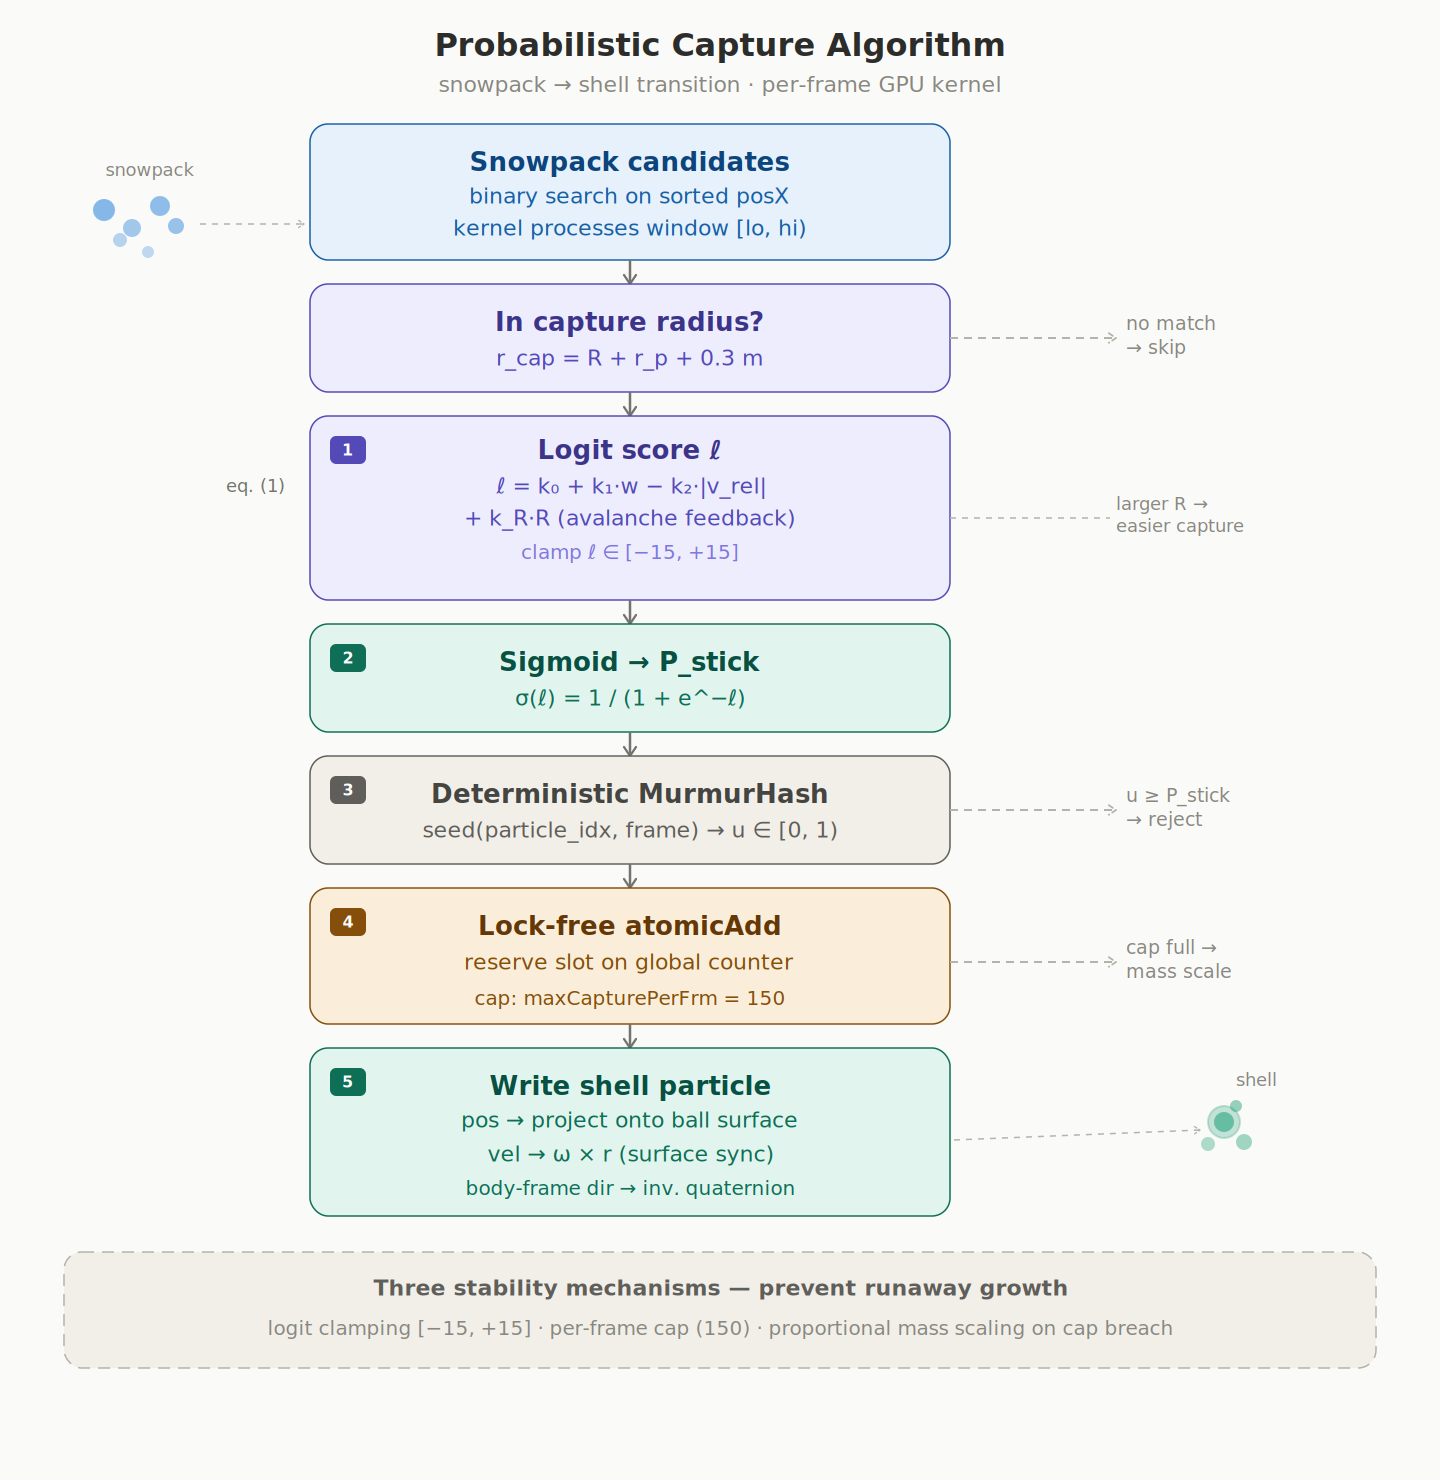
\includegraphics[width=0.9\columnwidth]{figures/capture_diagram.png}}
  \caption{The probabilistic capture algorithm overview. A binary search
  narrows the launch domain; each thread evaluates a sigmoid probability and
  reserves a shell slot via \texttt{atomicAdd} increasing the capacity.}
  \label{fig:capture}
\end{figure}

\subsection{Shell Particle Forces}
\label{sec:forces}

Each shell particle accumulates four force contributions:

\begin{enumerate}
  \item \textbf{Gravity}: $\mathbf{F}_g = m\,(0, -g, 0)$.
  \item \textbf{Mass-proportional damping}: $\mathbf{F}_d = -k_d \cdot m
        \cdot \mathbf{v}$.
  \item \textbf{Tether spring-damper} to the ball surface anchor:
        %
        \begin{equation}
          \mathbf{F}_{\text{tether}} = K(\mathbf{x}_{\text{tgt}} - \mathbf{x})
          + D(\mathbf{v}_{\text{tgt}} - \mathbf{v}),
          \label{eq:tether}
        \end{equation}
        %
        where the target position is computed from the ball's quaternion
        and each particle's body-frame attachment direction.
  \item \textbf{DEM contact} (computed in a separate collision kernel):
        soft-sphere penalty with Coulomb tangential friction
        ($|\mathbf{F}_t| \leq \mu_p |\mathbf{F}_n|$) and short-range
        cohesion for overlapping pairs.
\end{enumerate}

\subsection{Integration and Ground Collision}
\label{sec:integration}

A \textbf{semi-implicit (symplectic) Euler} scheme updates velocity then
position:
%
\begin{equation}
  \mathbf{v}^{n+1} = \mathbf{v}^n + \frac{\mathbf{F}}{m}\Delta t, \qquad
  \mathbf{x}^{n+1} = \mathbf{x}^n + \mathbf{v}^{n+1}\Delta t.
  \label{eq:euler}
\end{equation}
%
Ground collision resolves penetration against the inclined plane with normal
restitution ($e = 0.15$) and Coulomb friction ($\mu = 0.14$). When particles
are captured, the ball velocity is scaled to conserve linear momentum:
$\mathbf{v}' = \frac{m_{\text{old}}}{m_{\text{old}} + \Delta m}\,\mathbf{v}$.

% !TEX root = ../paper.tex
\section{System Architecture}
\label{sec:architecture}

The simulation state is partitioned into three cooperating subsystems, each
with distinct mutability semantics (Fig.~\ref{fig:architecture}).

\subsection{Snowpack (Static)}

The snowpack is a read-mostly Structure-of-Arrays (SoA) containing $10^6$
particles with positions, radii, masses, wetness values, and an \texttt{alive}
flag (\texttt{AVAILABLE}/\texttt{CONSUMED}). Positions are immutable after
initialisation; only the \texttt{alive} flag is toggled atomically upon
capture. The array is sorted once by \texttt{posX} to enable binary-search
range limiting.

\subsection{Shell (Dynamic)}

The shell is a fully dynamic SoA (\texttt{ParticleSystem}) storing positions,
velocities, forces, masses, radii, state flags, wetness, and body-frame
attachment vectors (\texttt{attachLocal}). Its capacity starts at 256 and
\textbf{grows dynamically} (doubling) as particles are captured, using
\texttt{cudaMalloc}/\texttt{cudaMemcpy} with the old buffer freed after copy.
Under steady-state conditions (1M snowpack, default parameters), the shell
stabilises at approximately 4{,}000 active particles.

\subsection{Core (Rigid Body)}

The snowball core is a single \texttt{SnowballState} struct maintained on the
host: position, velocity, quaternion orientation, angular velocity, mass, and
radius. It is updated each frame via rigid-body slope dynamics with rolling
and aerodynamic drag. Mass and radius grow as captured particles contribute
mass, with the radius derived as $R = (3m / 4\pi\rho)^{1/3}$.

\begin{figure}[H]
  \centering
  \fbox{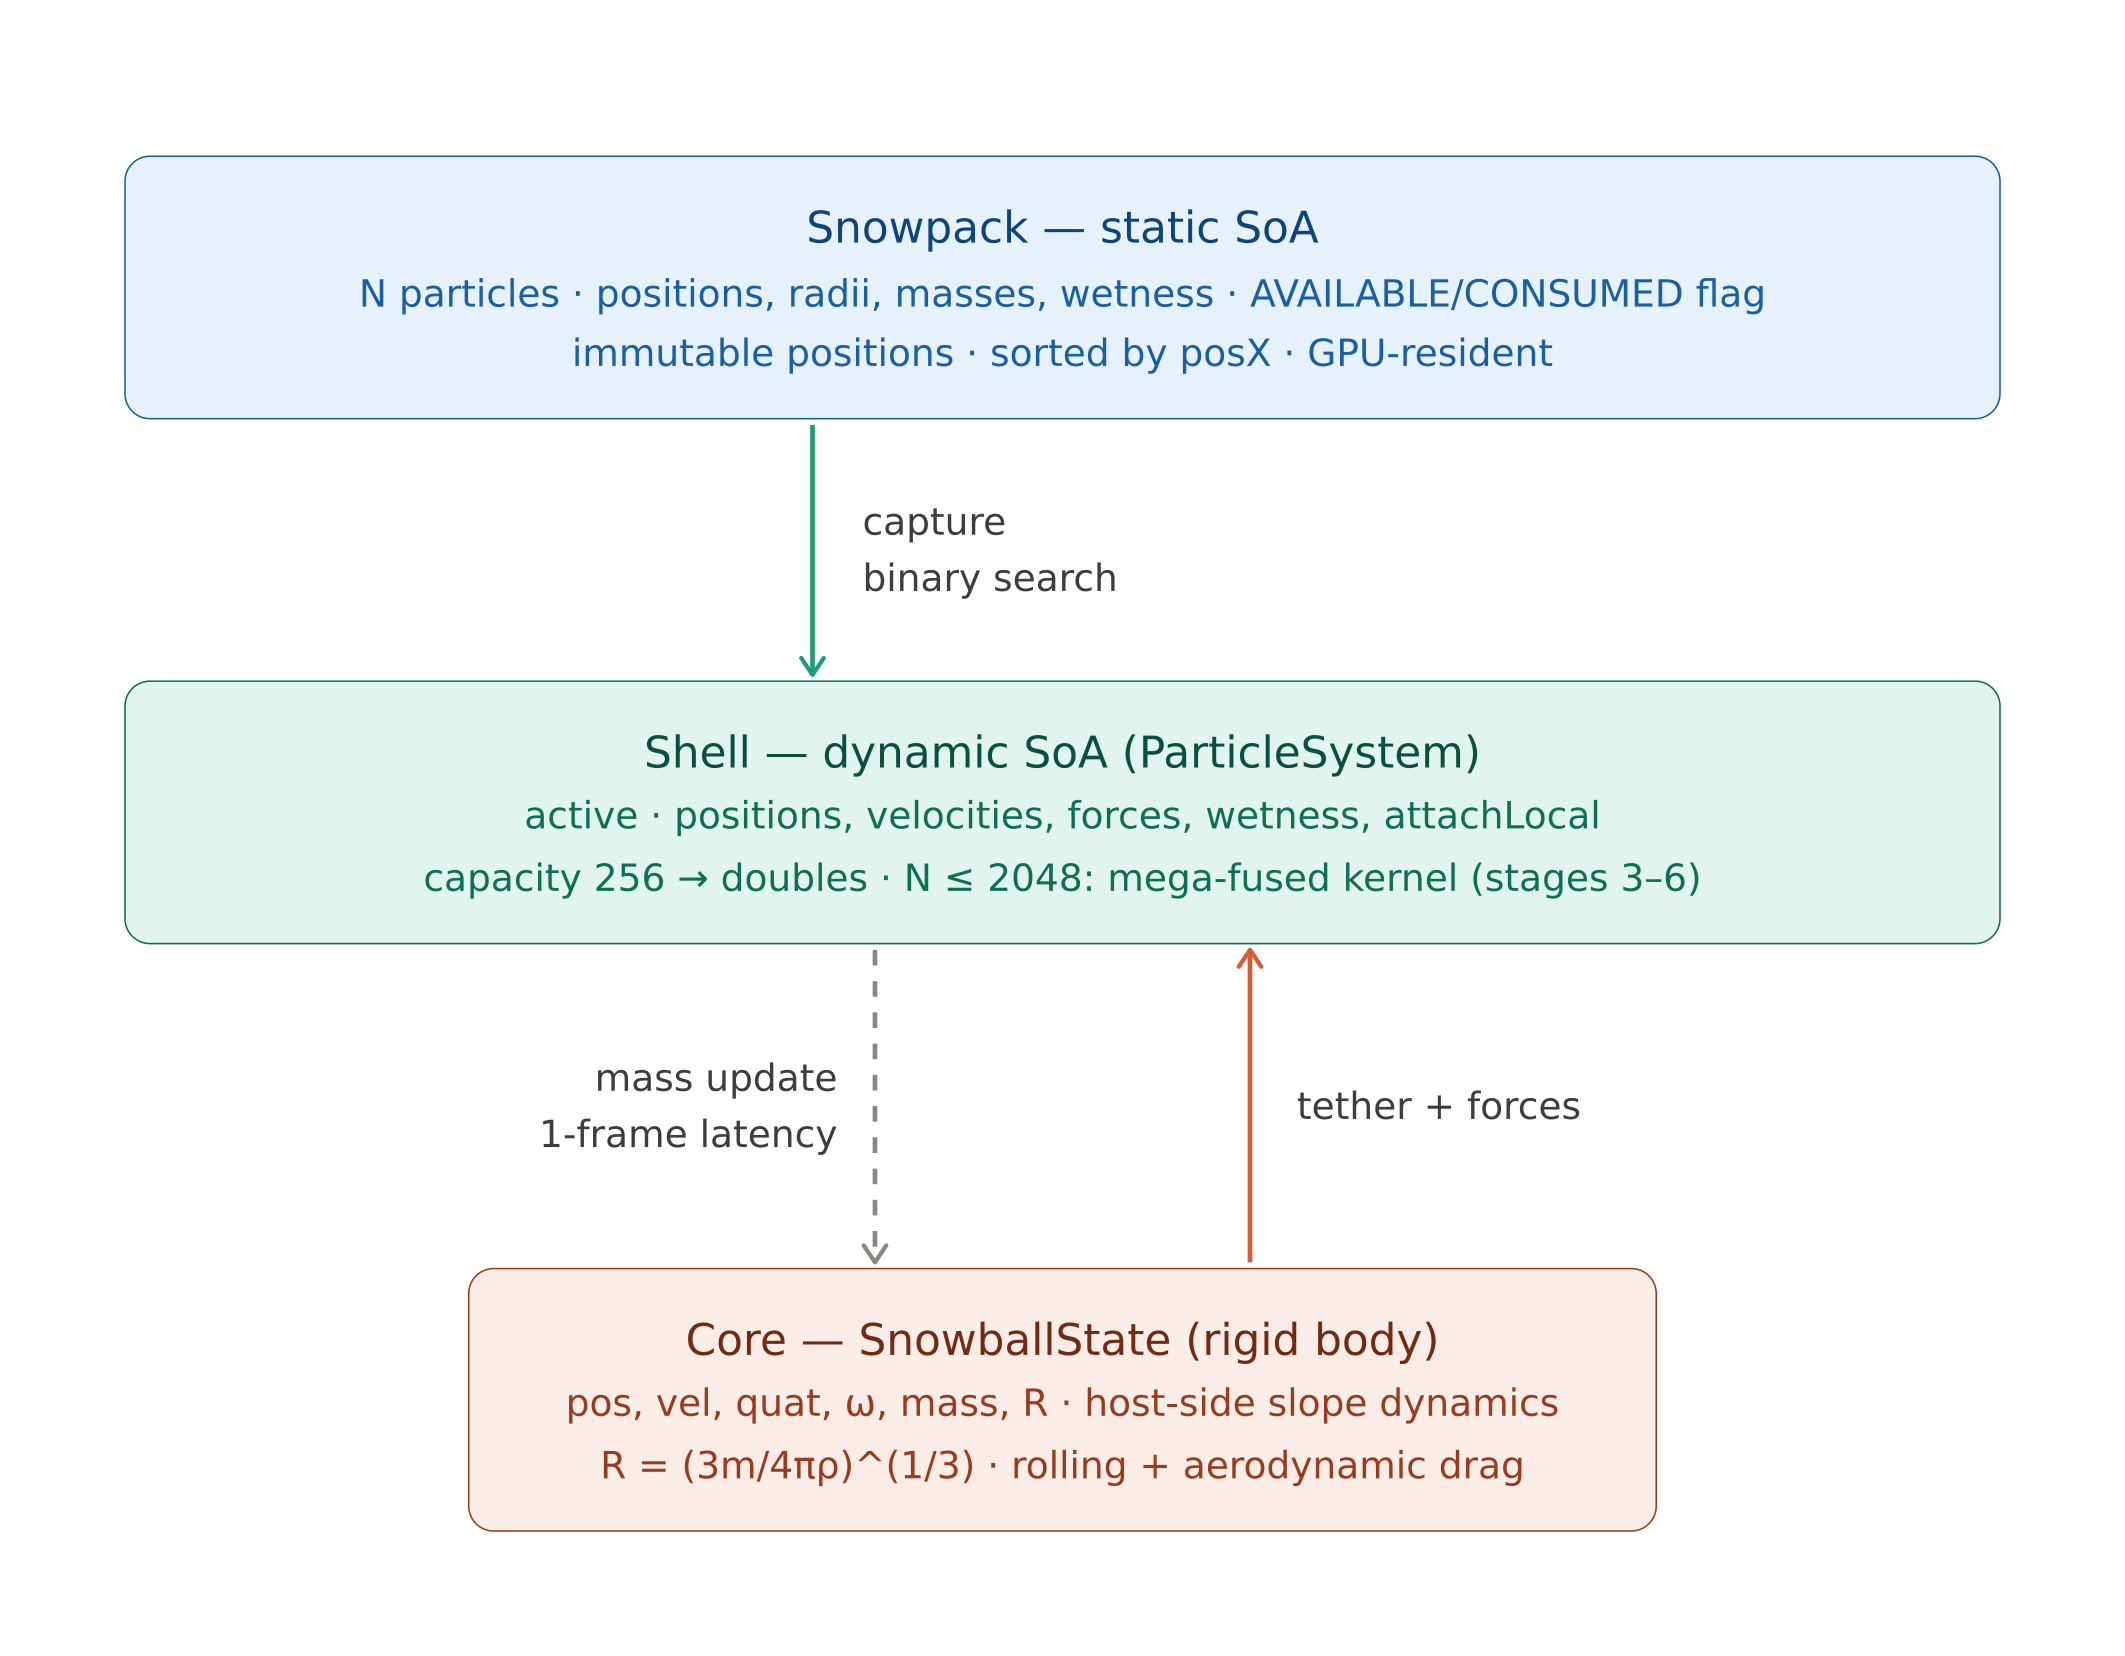
\includegraphics[width=0.9\columnwidth]{figures/architecture.png}}
  \caption{Three-tier particle architecture. The capture kernel converts
  snowpack particles into shell particles; each shell particle is tethered to
  the rigid-body core via a spring-damper.}
  \label{fig:architecture}
\end{figure}

\subsection{Per-Frame Data Flow}
\label{sec:dataflow}

The per-frame pipeline proceeds as follows:

\begin{enumerate}
  \item \textbf{Capture}: snowpack $\to$ shell (range-limited binary search).
  \item \textbf{Core mass update}: deferred readback (1-frame latency) of
        capture counters from device; momentum-conserving velocity scaling.
  \item \textbf{Forces + Tether}: gravity, damping, and tether spring
        (fused kernel).
  \item \textbf{Grid build}: spatial hash, CUB radix sort, cell ranges
        (\emph{parallel stream}).
  \item \textbf{Collision}: neighbour DEM + cohesion.
  \item \textbf{Integrate + Ground}: semi-implicit Euler + slope constraint
        (fused kernel).
  \item \textbf{Core rigid-body update}: host-side slope dynamics.
\end{enumerate}

For small shell counts ($N \leq 2048$), stages 3--6 are replaced by a
single \textbf{mega-fused kernel} that performs the entire physics pipeline
in one launch (Section~\ref{sec:mega_fused}).

\subsection{Deferred Capture Readback}
\label{sec:deferred}

Capture counters (particle count and accumulated mass) reside in a packed
8-byte device buffer, reset each frame via \texttt{cudaMemsetAsync}. The
result is read back asynchronously to pinned host memory. The host processes
the readback at the top of the \emph{next} frame (1-frame latency, physically
negligible at 300\,Hz). When more threads passed the probabilistic test than
the per-frame cap allows, the credited mass is scaled proportionally:
%
\begin{equation}
  m_{\text{credited}} = m_{\text{total}} \cdot
  \frac{\text{actualNew}}{\text{d\_captureCount}},
  \label{eq:mass_scaling}
\end{equation}
%
preventing the ball radius from inflating and triggering a runaway feedback
loop.

% !TEX root = ../paper.tex
\section{GPU Pipeline}
\label{sec:pipeline}

The GPU implementation provides two execution paths selected at runtime based
on the current shell particle count $N$. Both paths share the capture stage and
the host-side core update; they differ in how shell physics is dispatched.

\subsection{Large-$N$ Path ($N > 2048$)}
\label{sec:large_n}

Seven stages execute on two CUDA streams with fork/join synchronisation via
lightweight events (\texttt{cudaEventDisableTiming}):

\begin{table}[H]
  \caption{Large-$N$ GPU pipeline stages.}
  \label{tab:pipeline_large}
  \centering
  \scriptsize
  \begin{tabular}{@{}clccc@{}}
    \toprule
    \textbf{\#} & \textbf{Stage} & \textbf{Kernel} & \textbf{Stream} & \textbf{Block} \\
    \midrule
    1 & Capture         & \texttt{captureFromSnowpack}  & sim  & 256 \\
    2 & Core update     & host code                     & ---  & --- \\
    3 & Forces+Tether   & \texttt{forceTether}          & sim  & 256 \\
    4 & Grid build      & hash$\to$sort$\to$ranges      & grid & 256 \\
    5 & Collision       & \texttt{neighborCollision}    & sim  & 512 \\
    6 & Integrate+Ground& \texttt{integrateGround}      & sim  & 256 \\
    7 & Core RB         & host code                     & ---  & --- \\
    \bottomrule
  \end{tabular}
\end{table}

Stages 3 (forces\,+\,tether) and 4 (grid build) execute \textbf{concurrently}
on \texttt{simStream} and \texttt{gridStream}, respectively. The collision
kernel (stage~5) waits for both via \texttt{cudaStreamWaitEvent} on
\texttt{evGridDone}. Stream synchronisation events use
\texttt{cudaEventDisableTiming} to eliminate timing overhead (Section~\ref{sec:streams}).

\subsection{Small-$N$ Path ($N \leq 2048$)}
\label{sec:small_n}

When the shell count is small, the overhead of the grid build (5--8 GPU
commands: clear + hash + CUB sort + cell ranges) exceeds the computational
benefit. A single \textbf{mega-fused kernel} (\texttt{shellPhysicsFused})
replaces stages 3--6, reducing GPU commands per frame from $\sim$10 to
\textbf{1} and keeping all intermediate forces in registers
(Section~\ref{sec:mega_fused}).

\subsection{Block Sizes and \texttt{\_\_launch\_bounds\_\_}}
\label{sec:block_sizes}

Block sizes are chosen to balance \textbf{SM coverage} (all SMs receive at
least one block) against per-block resource consumption. With $N = 4{,}000$ and
5~SMs on the GTX~960M, a block of 1024 yields only $\lceil4000/1024\rceil = 4$
blocks, leaving 1~SM idle (20\% wasted). A block of 256 yields 16~blocks,
ensuring full coverage.

The \texttt{neighborCollisionKernel} uses block size 512 dictated by the
warp-cooperative tile layout ($\text{MAX\_WARPS} = 16 = 512/32$). All other
physics kernels use 256. Each kernel is annotated with
\texttt{\_\_launch\_bounds\_\_(maxThreads, minBlocks)} to guide the register
allocator (Table~\ref{tab:occupancy}).

\subsection{Adaptive Path Selection}
\label{sec:adaptive_path}

The $N = 2048$ threshold is chosen empirically: below this value, the
mega-fused kernel's reduced command overhead ($\sim$100--150\,$\mu$s) outweighs
the cost of brute-force $O(N^2)$ collision detection. Above 2048, the grid-based
$O(N \cdot k)$ path becomes more efficient despite the additional GPU commands.
At typical steady-state conditions ($N \approx 4{,}000$ particles), the grid path
executes $\sim$3--4 neighbours per particle, yielding $\sim$16{,}000 pair
evaluations compared to $\sim 16\text{M}$ in brute-force --- a $1000\times$
reduction that justifies the grid-build overhead.

% !TEX root = ../paper.tex
\section{GPU Optimizations}
\label{sec:optimizations}

This section details every GPU-level optimisation applied in the project,
with quantitative analysis of occupancy, bandwidth, and launch-overhead
trade-offs on Maxwell hardware (SM~5.0/5.3).

% ===================================================================
\subsection{Memory Coalescing via SoA Layout}
\label{sec:soa}

A warp of 32 threads issues a single memory transaction. With the
Structure-of-Arrays layout, threads 0--31 access contiguous floats and the
hardware merges the request into a single 128-byte transaction (100\%
efficiency). An Array-of-Structures layout would scatter accesses across
a stride equal to the struct size, wasting up to 90\% of bus bandwidth.

Indirect accesses introduced by the spatial grid
(\texttt{posX[particleIndex[s]]}) are not perfectly coalesced. However, after
CUB radix sort, particles within the same cell have nearby indices ---
loads are nearly coalesced and benefit from L2 cache reuse (the steady-state
working set of 4{,}000 particles fits in $\sim$128\,KB, or 12.5\% of the 1\,MB
L2 on the GTX~960M).

% ===================================================================
\subsection{Warp-Cooperative Shared-Memory Tiling}
\label{sec:tiling}

Shared memory is on-chip SRAM ($\sim$5-cycle latency, $\sim$1.3\,TB/s), compared
to global memory ($\sim$300--500 cycles, $\sim$30\,GB/s on Maxwell). The
\texttt{neighborCollisionKernel} employs \textbf{warp-cooperative tiling}: each
warp loads a tile of 32 neighbours into shared memory and all 32 threads read
from it. The tile is declared as \texttt{[MAX\_WARPS][WARP\_SIZE + 1]}, where
$\text{MAX\_WARPS} = 16 = 512/32$ and the \texttt{+1} padding avoids
shared-memory bank conflicts (successive warps access different banks):

\begin{lstlisting}
__shared__ float s_px[MAX_WARPS][WARP_SIZE+1];
__shared__ float s_py[MAX_WARPS][WARP_SIZE+1];
__shared__ float s_pz[MAX_WARPS][WARP_SIZE+1];
__shared__ float s_r [MAX_WARPS][WARP_SIZE+1];
__shared__ int   s_idx[MAX_WARPS][WARP_SIZE+1];
__shared__ int   s_state[MAX_WARPS][WARP_SIZE+1];
\end{lstlisting}

\textbf{Why \texttt{\_\_syncwarp()} instead of \texttt{\_\_syncthreads()}.}
The previous kernel used \texttt{\_\_syncthreads()} combined with symmetric
iteration. When excess threads executed an early \texttt{return} before the
barrier, the remaining threads deadlocked --- violating the CUDA specification
that \emph{all} threads in a block must reach the same
\texttt{\_\_syncthreads()}. The warp-scoped \texttt{\_\_syncwarp()} avoids this:
all 32 threads always participate in the tile load (the
\texttt{lane < tileLen} guard is a predicated branch, not an early return).

\textbf{Why velocities are not tiled.} Adding \texttt{s\_vx/vy/vz} would
increase per-block shared memory from $\sim$10.6\,KB to $\sim$17\,KB. At 3
resident blocks this exceeds the 48\,KB limit (51\,KB), reducing occupancy
from 75\% to 50\%. Velocities are instead loaded on-demand via
\texttt{\_\_ldg()} only when contact is detected, which is rare ($\sim$2--5
contacts out of 10--50 neighbours per cell).

% ===================================================================
\subsection{Atomic Reduction Strategy}
\label{sec:atomics}

On Maxwell, \texttt{atomicAdd} on FP32 generates a compare-and-swap (CAS) loop
that under contention executes 5--10 retry iterations. The previous symmetric
collision kernel (\texttt{j > i}) required 6~\texttt{atomicAdd} per pair.

The current design uses \textbf{full non-symmetric iteration}: every thread $i$
iterates over all neighbours $j \neq i$, accumulating forces entirely in
registers. The sole write is a direct store to
\texttt{forceX/Y/Z[i]} --- thread~$i$ is the only writer, so no atomic is
needed. This trades doubled FLOPs ($N$ vs.\ $N/2$ pair evaluations) for
\textbf{zero contention}, which is a net win on Maxwell where each CAS retry
costs 20--60 cycles versus $\sim$4 cycles for a direct store.

% ===================================================================
\subsection{Occupancy Tuning}
\label{sec:occupancy}

Occupancy is defined as the ratio of active warps to the maximum warps per SM
(64 on SM~5.0/5.3, i.e.\ 2048 threads). It is constrained by registers
(65{,}536/SM), shared memory (48\,KB/SM), and block count (max 32/SM).
Table~\ref{tab:occupancy} reports the per-kernel occupancy achieved.

\begin{table}[H]
  \caption{Per-kernel occupancy (\texttt{ptxas~-v} output).}
  \label{tab:occupancy}
  \centering
  \scriptsize
  \begin{tabular}{@{}lccccc@{}}
    \toprule
    \textbf{Kernel} & \textbf{Regs} & \textbf{Block} & \textbf{Blk/SM}
      & \textbf{Occ.} & \textbf{Limiter} \\
    \midrule
    \texttt{neighborCollision}    & 40 & 512 & 3 & 75.0\% & Shared mem. \\
    \texttt{forceTether}          & 27 & 256 & 8 & 100\%  & --- \\
    \texttt{integrateGround}      & 24 & 256 & 8 & 100\%  & --- \\
    \texttt{captureFromSnowpack}  & 48 & 256 & 5 & 62.5\% & Registers \\
    \texttt{shellPhysicsFused}    & 37 & 256 & 5 & 62.5\% & Registers \\
    \texttt{bruteForceCollision}  & 38 & 256 & 5 & 62.5\% & Registers \\
    \texttt{computeHash}          & 14 & 256 & 8 & 100\%  & --- \\
    \texttt{buildCellRanges}      &  7 & 256 & 8 & 100\%  & --- \\
    \texttt{clearPrevCells}       &  8 & 256 & 8 & 100\%  & --- \\
    \bottomrule
  \end{tabular}
\end{table}

All kernels report \textbf{zero register spill} in the \texttt{ptxas} output.
Four kernels operate below 100\%:

\begin{itemize}
  \item \textbf{\texttt{neighborCollision} (75\%)}: dual constraint --- 40
        regs $\times$ 512 $= 20{,}480$ regs/block ($\lfloor65536/20480\rfloor
        = 3$ blocks) and shared memory: $3 \times 12.4$\,KB $= 37$\,KB fits,
        but $4 \times 12.4$\,KB $= 49.6$\,KB exceeds 48\,KB.
  \item \textbf{\texttt{captureFromSnowpack} (62.5\%)}: 48 regs --- the
        highest in the project. The kernel computes \texttt{expf}, hash PRNG,
        3D distance, and quaternion rotation. Reaching 100\% would require 32
        regs (a 33\% cut), causing massive spill in a kernel that is already
        range-limited to $\sim$500--2{,}000 threads per frame.
  \item \textbf{\texttt{shellPhysicsFused} / \texttt{bruteForceCollision}
        (62.5\%)}: 37--38 regs + shared memory for brute-force tiling
        ($8 \times 257 \times 4$\,B $\approx 8$\,KB/block). At 6+ blocks
        shared memory exceeds budget. These kernels run only for
        $N \leq 2048$.
\end{itemize}

\textbf{Design principle: zero spill $>$ 100\% occupancy.} A single register
spill costs $\sim$300 cycles (DRAM round-trip), while one fewer warp costs
only a few scheduling cycles. For compute-bound kernels or kernels whose
working set fits in cache, keeping all variables in registers outweighs the
benefit of additional concurrent warps.

% ===================================================================
\subsection{Single Precision and Fast Math}
\label{sec:fp32}

Consumer Maxwell GPUs have an FP64\,:\,FP32 throughput ratio of 1\,:\,32.
With $\Delta t = 5$\,ms, the Euler truncation error
($O(\Delta t^2) \approx 2.5 \times 10^{-5}$) dominates FP32 rounding
($\epsilon \approx 6 \times 10^{-8}$) by three orders of magnitude, making
single precision entirely adequate. All literals are \texttt{f}-suffixed, all
math functions use \texttt{f}-variants (\texttt{sqrtf}, \texttt{expf},
\texttt{fmaxf}), and \texttt{M\_PI} is defined as \texttt{float}. The
\texttt{-{}-use\_fast\_math} flag enables fused operations and
flush-to-zero for denormals.

% ===================================================================
\subsection{\texttt{\_\_restrict\_\_} and \texttt{\_\_ldg()}}
\label{sec:ldg}

The \texttt{\_\_restrict\_\_} qualifier enables the compiler to reorder
loads/stores and cache values in registers. On SM $\geq$ 3.5,
\texttt{\_\_ldg()} routes loads through the read-only texture cache, which is
physically separate from the L1/shared memory used for read-write data. This
\textbf{doubles effective cache bandwidth} without conflicts. All physics and
grid kernels use explicit \texttt{\_\_ldg()} for immutable inputs; the capture
kernel uses \texttt{const \_\_restrict\_\_} pointers, which the compiler
auto-routes through the read-only cache at \texttt{-O3}.

% ===================================================================
\subsection{Constant Memory}
\label{sec:constant}

The \texttt{SimParams} struct ($\sim$152\,B) is placed in
\texttt{\_\_constant\_\_} memory. Its dedicated 64\,KB cache \textbf{broadcasts}
a single value to all 32 threads in a warp in $\sim$5 cycles, without consuming
registers. Physics constants (gravity, stiffness, damping, etc.) are read
identically by all threads --- a perfect broadcast use-case. The struct is
uploaded once at startup via \texttt{cudaMemcpyToSymbol}.

% ===================================================================
\subsection{Kernel Fusion}
\label{sec:fusion}

Two pairs of kernels were fused to eliminate global-memory round-trips:

\begin{itemize}
  \item \texttt{applyForces} + \texttt{shellCoreTether} $\to$
        \textbf{\texttt{forceTether}}: eliminates one round-trip for
        \texttt{forceX/Y/Z}.
  \item \texttt{integrate} + \texttt{groundCollision} $\to$
        \textbf{\texttt{integrateGround}}: eliminates one round-trip for
        position/velocity.
\end{itemize}

Fusion keeps intermediate results in registers rather than writing to global
memory and re-reading in a second kernel.

% ===================================================================
\subsection{Spatial Hashing and CUB Radix Sort}
\label{sec:spatial_hash}

Collision detection is reduced from $O(N^2)$ to $O(N \cdot k)$ via
uniform-grid spatial hashing~\cite{teschner2003}. The hash function uses
prime multiplication: $h = (c_x \cdot 73856093) \oplus (c_y \cdot 19349663)
\oplus (c_z \cdot 83492791)$ with additional bit-mixing, masked to a compact
table of size $\texttt{nextPowerOf2}(N \times 8)$. This reduces memory from
$\sim$75\,MB (full domain) to $\sim$256\,KB.

CUB \texttt{DeviceRadixSort::SortPairs} sorts (hash, particleIndex) pairs with
a pre-allocated temporary buffer and bit-count limited to
$\lceil\log_2(\text{tableSize})/4\rceil \times 4$ to minimise radix passes.
A \texttt{clearPrevCellsKernel} clears only cells used in the previous frame
(scatter-clear), avoiding a full-array \texttt{memset}.

% ===================================================================
\subsection{Sorted Snowpack and Binary-Search Capture}
\label{sec:binary_search}

The snowpack is static --- sorting it once at initialisation by \texttt{posX}
enables a host-side \texttt{std::lower\_bound}/\texttt{upper\_bound} each frame
to find the interval $[\text{lo}, \text{hi})$ within capture distance. The
kernel launches on this subset only, reducing threads from $10^6$ to
$\sim$500--2{,}000 (a 50--100$\times$ reduction). The host-side binary search
costs $\sim$1\,$\mu$s on the pinned sorted array.

% ===================================================================
\subsection{Mega-Fused Kernel for Small $N$}
\label{sec:mega_fused}

With $N \leq 2048$, the standard pipeline requires $\sim$10 GPU commands per
frame, adding $\sim$100--150\,$\mu$s of pure launch overhead on the GTX~960M
(each command incurs $\sim$10--15\,$\mu$s driver overhead). A single
\textbf{\texttt{shellPhysicsFusedKernel}} replaces the entire pipeline: gravity
$\to$ damping $\to$ tether $\to$ brute-force $O(N^2)$ collision $\to$ Euler
integration $\to$ ground collision. Forces \textbf{never transit through global
memory} --- they stay in registers throughout. At $N = 2048$, brute-force
collision is $4 \times 10^6$ iterations ($\sim$0.3\,ms), still well within
budget. Above 2048 the grid-based $O(N \cdot k)$ path becomes more efficient.

% ===================================================================
\subsection{Pinned Memory for Asynchronous Copies}
\label{sec:pinned}

Nsight Systems profiling revealed 30--40\,ms GPU stalls caused by
\texttt{cudaMemcpyAsync} targeting \textbf{pageable} host memory --- the driver
silently inserts a device-wide synchronisation. All host buffers for async
readback are now allocated with \texttt{cudaMallocHost} (pinned memory):
capture counters, sorted \texttt{posX}, and trace buffers. Additionally,
the capture count (int) and mass (float) are packed into a single 8-byte
buffer, reducing per-frame GPU commands from 4 to 2 ($\sim$20--30\,$\mu$s
saved).

% ===================================================================
\subsection{Multi-Stream Pipeline}
\label{sec:streams}

Physics and grid-build kernels run on dedicated non-blocking CUDA streams.
\texttt{simStream} executes forces $\to$ collision $\to$ integration;
\texttt{gridStream} builds the spatial hash in parallel with force computation.
An additional third \texttt{traceStream} handles asynchronous device-to-host 
copies for optional trace snapshots. Fork/join is implemented via
\texttt{cudaEventRecord}/\texttt{cudaStreamWaitEvent} with timing-disabled
events to minimise overhead.

\begin{figure}[H]
  \centering
  \fbox{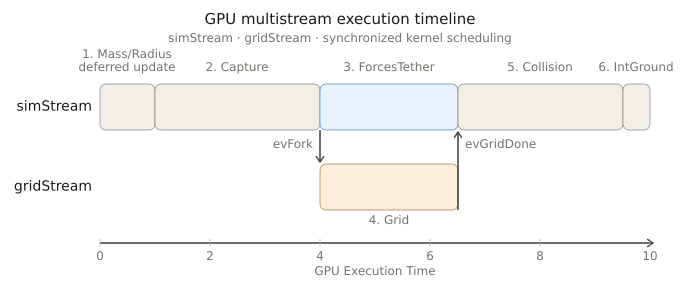
\includegraphics[width=0.9\columnwidth]{figures/multistream.png}}
  \caption{Dual-stream pipeline. Stages~3 and~4 overlap on separate streams;
  stage~5 waits for both via a lightweight CUDA event.}
  \label{fig:pipeline}
\end{figure}

% ===================================================================
\subsection{Gated Event Recording}
\label{sec:gated_events}

Each \texttt{cudaEventRecord()} call incurs $\sim$10--15\,$\mu$s driver
overhead. With up to 14 event records per frame (start\,+\,end for 7
timing pairs), this adds $\sim$110--165\,$\mu$s per frame. Events are recorded
only every \texttt{TIMING\_INTERVAL\,=\,64} frames (or when logging/rendering
is active). The 63~non-profiled frames save $\sim$12 event records each.
Synchronisation events (\texttt{evFork}, \texttt{evGridDone}) are always
recorded since they are required for correctness.

% ===================================================================
\subsection{ALU Optimizations}
\label{sec:alu}

\begin{itemize}
  \item \textbf{\texttt{rsqrtf} pattern}: $1/\sqrt{x}$ in a single SFU cycle
        ($\sim$8 cycles), then \texttt{dist = dist2 * invDist} (1 FMA), saving
        one SFU op compared to \texttt{sqrtf + 1.0f/dist}.
  \item \textbf{Tangential friction}: squared-magnitude threshold
        (\texttt{vt2 > 1e-16f}) with \texttt{rsqrtf(vt2)} avoids a separate
        \texttt{sqrtf} + division.
  \item \textbf{Branchless clamping}: \texttt{fmaxf(f\_spring - f\_damp, 0.0f)}
        compiles to a single \texttt{FMNMX} instruction (1~cycle) on Maxwell.
  \item \textbf{Hash-based PRNG}: a murmurhash variant (6 integer ops) replaces
        \texttt{curand} in the capture kernel, eliminating 48\,B/thread of
        global-memory state.
  \item \textbf{Quaternion rotation}: the Rodrigues formula uses 15 FMA
        operations versus 27 for a 3$\times$3 matrix multiply, and avoids
        constructing a temporary matrix (9 registers).
\end{itemize}

% ===================================================================
\subsection{Unity Build and Constant Sharing}
\label{sec:unity}

All GPU source files (\texttt{grid.cu}, \texttt{simulation.cu},
\texttt{snowpack.cu}) are \texttt{\#include}d into a single translation unit
\texttt{gpu\_unity.cu}. This shares the \texttt{\_\_constant\_\_ SimParams
d\_params} declaration across all kernels without separate compilation,
avoiding device-link overhead.

% ===================================================================
\subsection{Memory Hierarchy Summary}
\label{sec:mem_hierarchy}

Table~\ref{tab:mem_hierarchy} summarises how each memory level is exploited.

\begin{table}[H]
  \caption{Memory hierarchy utilisation.}
  \label{tab:mem_hierarchy}
  \centering
  \scriptsize
  \begin{tabular}{@{}lll@{}}
    \toprule
    \textbf{Level} & \textbf{Usage} & \textbf{Size} \\
    \midrule
    Registers        & Local vars, force accumulators & 24--48/thread \\
    \texttt{\_\_constant\_\_} & \texttt{SimParams} (broadcast) & $\sim$152\,B \\
    Shared memory    & Warp-cooperative tile          & 12.4\,KB/blk \\
    Read-only cache  & \texttt{\_\_ldg()} loads (immutable SoA fields)        & HW-managed \\
    L2 cache         & Particle working set           & 1\,MB / 256\,KB \\
    Global (GDDR5)   & SoA arrays                     & $16N \times 4$\,B \\
    \bottomrule
  \end{tabular}
\end{table}

\subsection{Holistic Optimization Strategy}
\label{sec:holistic}

The optimizations described above are not applied independently, but as an
integrated strategy responding to Maxwell's specific constraints. Register
pressure is minimized through constant memory (broadcasts), tiling (shared-memory
reuse), and fusion (avoiding intermediate global writes). This architecture-aware
methodology ensures that every optimization decision is motivated by profiling data
and hardware-specific trade-offs, rather than generic best practices.

% !TEX root = ../paper.tex
\section{CPU Reference Implementations}
\label{sec:cpu}

Two CPU builds mirror the GPU physics pipeline, enabling direct speedup
measurements against the same simulation logic. No rendering capabilities are included in these builds.

\subsection{SISD Baseline}

The scalar build (\texttt{AngrySanta\_SISD}) is compiled with all compiler
optimisations disabled (\texttt{-O0}, \texttt{/Od}), no inlining, no
auto-vectorisation, and no loop unrolling. It serves as a strict performance
floor for measuring both GPU and SIMD speedups. The simulation loop in
\texttt{simulation\_CPU.cpp} executes the same pipeline: capture $\to$
forces\,+\,tether $\to$ grid $\to$ collision $\to$ integrate\,+\,ground $\to$
core update.

\subsection{SIMD + OpenMP}

The optimized build (\texttt{AngrySanta\_SIMD}) uses SSE2 intrinsics on x86-64
and NEON intrinsics on ARM64, plus the OpenMP directives for multi-threading.
The SIMD implementation is portable across both platforms, with conditional
compilation to include the appropriate headers and define platform-specific macros:

\begin{lstlisting}
#if defined(__x86_64__) || defined(_M_X64)
  #include <immintrin.h>   // SSE / SSE2
  #define CPU_SIMD_X86 1
#elif defined(__aarch64__)
  #include <arm_neon.h>    // NEON
  #define CPU_SIMD_NEON 1
#endif
\end{lstlisting}

Each physics function processes 4 particles per iteration (128-bit SIMD lanes)
with a scalar remainder loop for the $N \bmod 4$ tail. SoA arrays are allocated
with 16-byte alignment (via platform-specific \texttt{\_aligned\_malloc} /
\texttt{aligned\_alloc} macros) to enable aligned packed loads
(\texttt{\_mm\_load\_ps} / \texttt{vld1q\_f32}).

\begin{lstlisting}
// In SIMD builds, allocate 16-byte aligned memory for packed loads/stores.
#ifdef SIMD
  #ifdef _MSC_VER
    #define ALLOC(bytes)  _aligned_malloc((bytes), 16)
    #define FREE(ptr)     _aligned_free(ptr)
  #else
    static inline void* simd_alloc_impl_(size_t bytes) {
      size_t aligned = (bytes + 15u) & ~(size_t)15u;
      return aligned_alloc(16, aligned > 0 ? aligned : 16);
    }
    #define ALLOC(bytes)  simd_alloc_impl_(bytes)
    #define FREE(ptr)     free(ptr)
  #endif
#else
  #define ALLOC(bytes)  malloc(bytes)
  #define FREE(ptr)     free(ptr)
#endif
\end{lstlisting}

When compiled with \texttt{-DHAS\_OPENMP}, data-parallel loops use
\texttt{\#pragma omp parallel for schedule(static)} for multi-threaded
distribution across CPU cores, applying to initialisation, force computation,
and integration. The only algorithmic difference is ~no spatial hashing --- 
collision detection remains $O(N^2)$ brute-force. This ensures that GPU speedup 
measurements isolate parallelization and architectural advantage rather than 
algorithmic improvements, and allows direct quantification of SIMD vs.~GPU performance.
% !TEX root = ../paper.tex
\section{Experimental Results}
\label{sec:results}

\subsection{Experimental Setup}

\begin{table}[H]
  \caption{Hardware specifications of the two test platforms.}
  \label{tab:hardware}
  \centering
  \scriptsize
  \begin{tabular}{@{}lcc@{}}
    \toprule
    & \textbf{Laptop (Windows)} & \textbf{Jetson Nano (Linux)} \\
    \midrule
    Host CPU           & Intel i7-6700HQ & ARM Cortex-A57 (SoC) \\
    CPU cores / threads & 4 / 8 & 4 / 4 \\
    GPU                & GeForce GTX 960M & Tegra X1 \\
    Compute capability & SM 5.0 & SM 5.3 \\
    VRAM               & 4\,GB & 4\,GB \\
    SMs                & 5      & 1 \\
    CUDA cores / SM    & 128    & 128 \\
    Total CUDA cores   & 640    & 128 \\
    L2 cache           & 1\,MB  & 256\,KB \\
    Memory             & 4\,GB GDDR5 & 4\,GB LPDDR4 (shared) \\
    Memory bandwidth   & $\sim$30\,GB/s & $\sim$25.6\,GB/s \\
    \bottomrule
  \end{tabular}
\end{table}

\subsection{GTX960M Per-Kernel Timing Physics Scenario}

These scenarios use a small number of particles ($N = 10^5$)
causing the simulation on GPU to remain in the fused regime.

\begin{table}[H]
  \caption{Wet snow. \\-}
  \label{tab:gtx_scenario1_timing}
  \centering
  \scriptsize
  \begin{tabular}{@{}lcccccc@{}}
    \toprule
    \textbf{Kernel} & \textbf{SISD (ms)} & \textbf{SIMD (ms)} & \textbf{GPU (ms)} \\
    \midrule
    captureFromSnowpack           & 0.0589 & 0.0568 & 0.0960 \\
    forceTether                   & 0.0091 & 0.0101 & 0.0000 \\
    shellGrid                     & 0.0365 & 0.0335 & 0.0000 \\
    bruteForceCollision           & 0.0904 & 0.0184 & 0.0000 \\
    integrateGround               & 0.0055 & 0.0101 & 0.0000 \\
    shellPhysicsFused             & 0.0000 & 0.0000 & 0.0846 \\
    coreUpdate                    & 0.0002 & 0.0001 & 0.0000 \\
    Overhead                      & 0.0005 & 0.0004 & 0.0414 \\
    \bottomrule
    FPS                           & 4975.2 & 7723.4 & 4503.9
  \end{tabular}
\end{table}

\begin{table}[H]
  \caption{Dry snow.\\--wetness-max 0.3 --stick-k1 3.0}
  \label{tab:gtx_scenario2_timing}
  \centering
  \scriptsize
  \begin{tabular}{@{}lccc@{}}
    \toprule
    \textbf{Kernel} & \textbf{SISD (ms)} & \textbf{SIMD (ms)} & \textbf{GPU (ms)} \\
    \midrule
    captureFromSnowpack           & 0.0345 & 0.0413 & 0.0765 \\
    forceTether                   & 0.0047 & 0.0083 & 0.0000 \\
    shellGrid                     & 0.0170 & 0.0227 & 0.0000 \\
    bruteForceCollision           & 0.0394 & 0.0086 & 0.0000 \\
    integrateGround               & 0.0029 & 0.0082 & 0.0000 \\
    shellPhysicsFused             & 0.0000 & 0.0000 & 0.0583 \\
    coreUpdate                    & 0.0001 & 0.0001 & 0.0000 \\
    Overhead                      & 0.0005 & 0.0004 & 0.0338 \\
    \bottomrule
    FPS                           & 10077.4 & 11174.3 & 5933.1
  \end{tabular}
\end{table}

\begin{table}[H]
  \caption{\centering Amplified avalanche feedback. \\ \centering --stick-rboost 10.0}
  \label{tab:gtx_scenario3_timing}
  \centering
  \scriptsize
  \begin{tabular}{@{}lccc@{}}
    \toprule
    \textbf{Kernel} & \textbf{SISD (ms)} & \textbf{SIMD (ms)} & \textbf{GPU (ms)} \\
    \midrule
    captureFromSnowpack           & 0.0508 & 0.0519 & 0.1108 \\
    forceTether                   & 0.0102 & 0.0098 & 0.0000 \\
    shellGrid                     & 0.0435 & 0.0369 & 0.0000 \\
    bruteForceCollision           & 0.1094 & 0.0243 & 0.0000 \\
    integrateGround               & 0.0062 & 0.0100 & 0.0000 \\
    shellPhysicsFused             & 0.0000 & 0.0000 & 0.1011 \\
    coreUpdate                    & 0.0001 & 0.0001 & 0.0000 \\
    Overhead                      & 0.0005 & 0.0004 & 0.0485 \\
    \bottomrule
    FPS                           & 4529.0 & 7491.9 & 3839.4
  \end{tabular}
\end{table}

\begin{table}[H]
  \caption{High inter-particle friction. \\ --part-friction 0.6}
  \label{tab:gtx_scenario4_timing}
  \centering
  \scriptsize
  \begin{tabular}{@{}lccc@{}}
    \toprule
    \textbf{Kernel} & \textbf{SISD (ms)} & \textbf{SIMD (ms)} & \textbf{GPU (ms)} \\
    \midrule
    captureFromSnowpack           & 0.0656 & 0.0932 & 0.0924 \\
    forceTether                   & 0.0096 & 0.0275 & 0.0000 \\
    shellGrid                     & 0.0394 & 0.0442 & 0.0000 \\
    bruteForceCollision           & 0.0934 & 0.0288 & 0.0000 \\
    integrateGround               & 0.0058 & 0.0148 & 0.0000 \\
    shellPhysicsFused             & 0.0000 & 0.0000 & 0.0887 \\
    coreUpdate                    & 0.0002 & 0.0002 & 0.0000 \\
    Overhead                      & 0.0007 & 0.0005 & 0.0440 \\
    \bottomrule
    FPS                           & 4657.1 & 4783.6 & 4442.7
  \end{tabular}
\end{table}

\begin{table}[H]
  \caption{Slope 45°.\\ --slope 45.0}
  \label{tab:gtx_scenario5_timing}
  \centering
  \scriptsize
  \begin{tabular}{@{}lccc@{}}
    \toprule
    \textbf{Kernel} & \textbf{SISD (ms)} & \textbf{SIMD (ms)} & \textbf{GPU (ms)} \\
    \midrule
    captureFromSnowpack           & 0.0454 & 0.0641 & 0.1035 \\
    forceTether                   & 0.0073 & 0.0135 & 0.0000 \\
    shellGrid                     & 0.0274 & 0.0338 & 0.0000 \\
    bruteForceCollision           & 0.0618 & 0.0163 & 0.0000 \\
    integrateGround               & 0.0045 & 0.0138 & 0.0000 \\
    shellPhysicsFused             & 0.0000 & 0.0000 & 0.0716 \\
    coreUpdate                    & 0.0002 & 0.0002 & 0.0000 \\
    Overhead                      & 0.0007 & 0.0005 & 0.0431 \\
    \bottomrule
    FPS                           & 6791.4 & 7035.4 & 4583.0
  \end{tabular}
\end{table}

\begin{figure}[H]
  \centering
  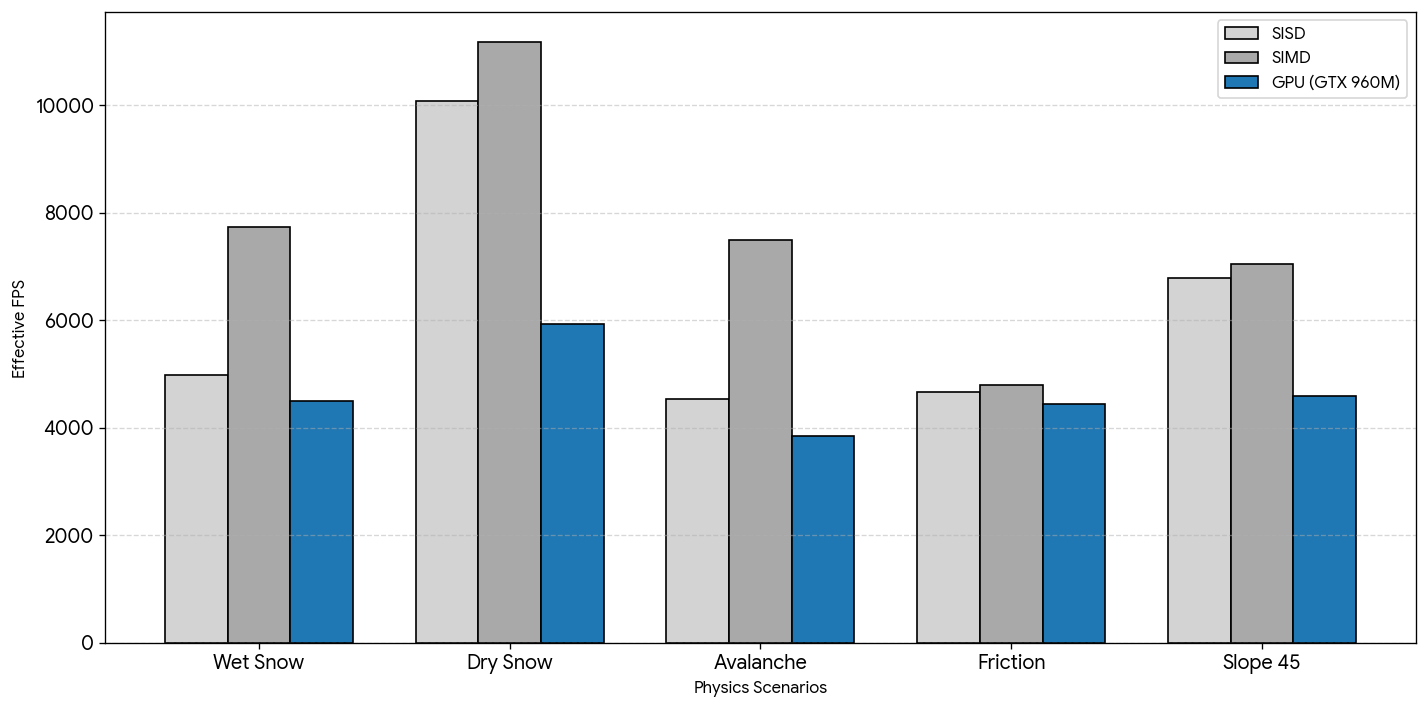
\includegraphics[width=\columnwidth]{figures/GTX_scenariocomparison.png}
  \caption{FPS comparison across the 5 physics scenarios on the GTX960M.}
  \label{fig:gtx_scenariocomparison}
\end{figure}

At $N = 10^5$ the GTX960M consistently yields lower FPS than both CPU 
baselines across all five physics scenarios. The root cause is a structural 
overhead problem: the shell layer never  grows beyond $\sim$2\,048 particles 
at this scale, so the \texttt{shellPhysicsFused} kernel executes in a single 
thread-block and occupies only one of the five available SMs.
The remaining GPU idle time is dominated by fixed costs---CUDA kernel
launch latency (${\sim}5\,\mu$s per kernel), host-device event
synchronization, and PCIe memory transfers---that together account for
roughly \textbf{35--50\%} of total frame time.\\
The i7-6700HQ, by contrast, executes the equivalent sequential physics loop
with minimal IPC stalls, benefiting from its deep out-of-order pipeline and
large L3 cache that keeps the $10^5$-particle snowpack entirely in cache.
SIMD further accelerates the CPU path through 4-wide AVX vectorisation of the
per-particle force loop, reaching peak FPS in the dry-snow scenario
(11\,174\,FPS) where the brute-force collision work is lightest.
\\
These results highlight an important design principle: GPU parallelism only
pays off once the workload is large enough to amortize launch and transfer
overheads. The crossover point is explored in the next section and occurs 
between $N = 100{,}000$ and $N = 500{,}000$ on this platform.

\subsection{Scaling with Particle Count}

\begin{table}[H]
  \caption{$N = 500{,}000$.}
  \label{tab:GTX_scaling_500k}
  \centering
  \scriptsize
  \begin{tabular}{@{}lccc@{}}
    \toprule
    \textbf{Kernel} & \textbf{SIMD (ms)} & \textbf{GPU (ms)} \\
    \midrule
    captureFromSnowpack        & 0.2293 & 0.0895 \\
    forceTether                & 0.0098 & 0.0143 \\
    shellGrid                  & 0.1753 & 0.0126 \\
    neighborCollision          & 0.1601 & 0.0297 \\
    integrateGround            & 0.0104 & 0.0021 \\
    shellPhysicsFused          & 0.0000 & 0.1348 \\
    coreUpdate                 & 0.0001 & 0.0000 \\
    Overhead                   & 0.0008 & 0.0398 \\
    \bottomrule
    FPS                        & 1706.6 & 3097.8 \\
  \end{tabular}
\end{table}

\begin{table}[H]
  \caption{$N = 1{,}000{,}000$.}
  \label{tab:GTX_scaling_1m}
  \centering
  \scriptsize
  \begin{tabular}{@{}lcc@{}}
    \toprule
    \textbf{Kernel} & \textbf{SIMD (ms)} & \textbf{GPU (ms)} \\
    \midrule
    captureFromSnowpack        & 0.6353 & 0.1038 \\
    forceTether                & 0.0192 & 0.0276 \\
    shellGrid                  & 0.4268 & 0.0538 \\
    neighborCollision          & 0.6570 & 0.0837 \\
    integrateGround            & 0.0596 & 0.0039 \\
    shellPhysicsFused          & 0.0000 & 0.0904 \\
    coreUpdate                 & 0.0002 & 0.0000 \\
    Overhead                   & 0.0010 & 0.0528 \\
    \bottomrule
    FPS                        & 555.8 & 2404.5 \\
  \end{tabular}
\end{table}

\begin{table}[H]
  \caption{$N = 5{,}000{,}000$.}
  \label{tab:GTX_scaling_5m}
  \centering
  \scriptsize
  \begin{tabular}{@{}lcc@{}}
    \toprule
    \textbf{Kernel} & \textbf{SIMD (ms)} & \textbf{GPU (ms)} \\
    \midrule
    captureFromSnowpack        &  3.9422 & 0.1653 \\
    forceTether                &  0.1069 & 0.0824 \\
    shellGrid                  &  3.1953 & 0.1927 \\
    neighborCollision          &  8.7393 & 0.9272 \\
    integrateGround            &  0.1052 & 0.0212 \\
    shellPhysicsFused          &  0.0000 & 0.0322 \\
    coreUpdate                 &  0.0004 & 0.0000 \\
    Overhead                   &  0.0015 & 0.0833 \\
    \bottomrule
    FPS                        & 62.1 & 664.7 \\
  \end{tabular}
\end{table}

\begin{table}[H]
  \caption{$N = 10{,}000{,}000$.}
  \label{tab:GTX_scaling_10m}
  \centering
  \scriptsize
  \begin{tabular}{@{}lcc@{}}
    \toprule
    \textbf{Kernel} & \textbf{SIMD (ms)} & \textbf{GPU (ms)} \\
    \midrule
    captureFromSnowpack        &  7.5114 & 0.2210 \\
    forceTether                &  0.2245 & 0.1363 \\
    shellGrid                  &  7.7466 & 0.2977 \\
    neighborCollision          & 26.8500 & 2.6099 \\
    integrateGround            &  0.1709 & 0.0484 \\
    shellPhysicsFused          &  0.0000 & 0.0192 \\
    coreUpdate                 &  0.0004 & 0.0000 \\
    Overhead                   &  0.0015 & 0.1031 \\
    \bottomrule
    FPS                        & 23.5 & 291.1 \\
  \end{tabular}
\end{table}

\begin{table}[H]
  \caption{GPU vs.\ SIMD CPU scaling with size $N$.}
  \label{tab:GTX_scaling}
  \centering
  \scriptsize
  \begin{tabular}{@{}rccccc@{}}
    \toprule
    \textbf{N} & \textbf{SIMD (FPS)} & \textbf{GPU (FPS)} & \textbf{SIMD (ms/f)} & \textbf{GPU (ms/f)} & \textbf{Speedup} \\
    \midrule
       500{,}000 & 1{,}706.6 & 3{,}097.8 & 0.586 & 0.323 & 1.8$\times$ \\
     1{,}000{,}000 &   555.8 & 2{,}404.5 & 1.799 & 0.416 & 4.3$\times$ \\
     5{,}000{,}000 &    62.1 &   664.7   & 16.10 & 1.505 & 10.7$\times$ \\
    10{,}000{,}000 &    23.5 &   291.1   & 42.55 & 3.435 & 12.4$\times$ \\
    \bottomrule
  \end{tabular}
\end{table}

\begin{figure}[H]
  \centering
  \fbox{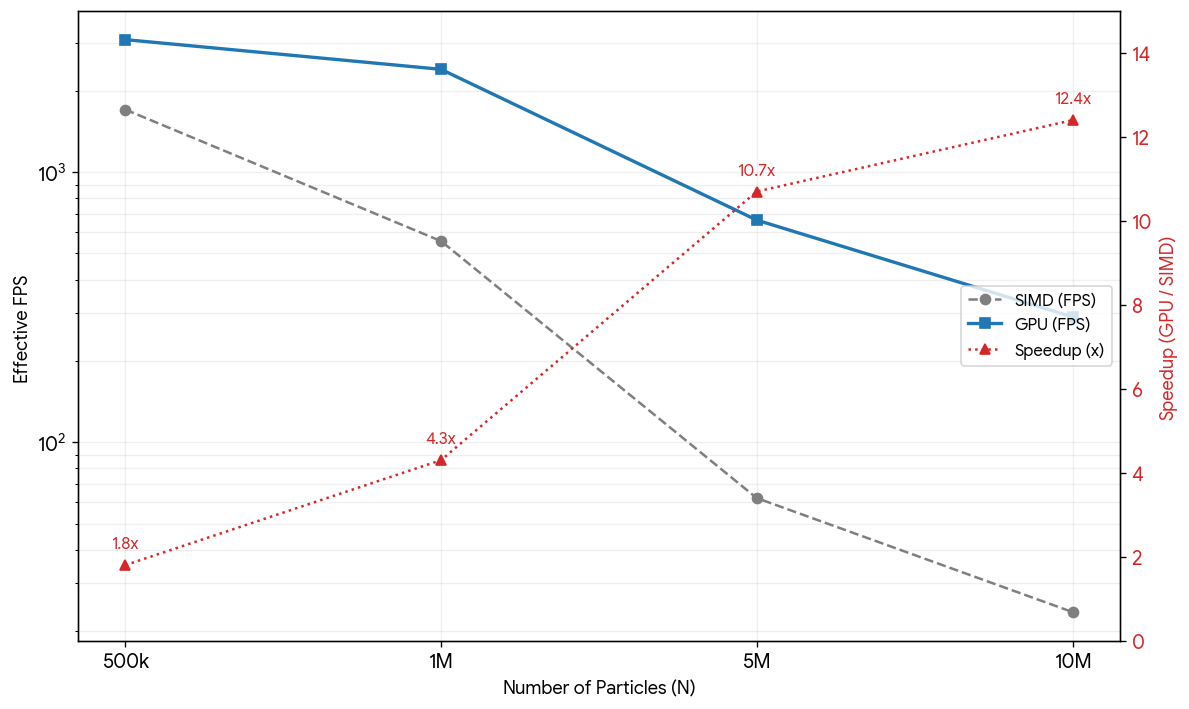
\includegraphics[width=0.9\columnwidth]{figures/GTX_scalingFPS.png}}
  \caption{Scaling: FPS SIMD CPU vs GTX960M.}
  \label{fig:GTX_scalingFPS}
\end{figure}

\begin{figure}[H]
  \centering
  \fbox{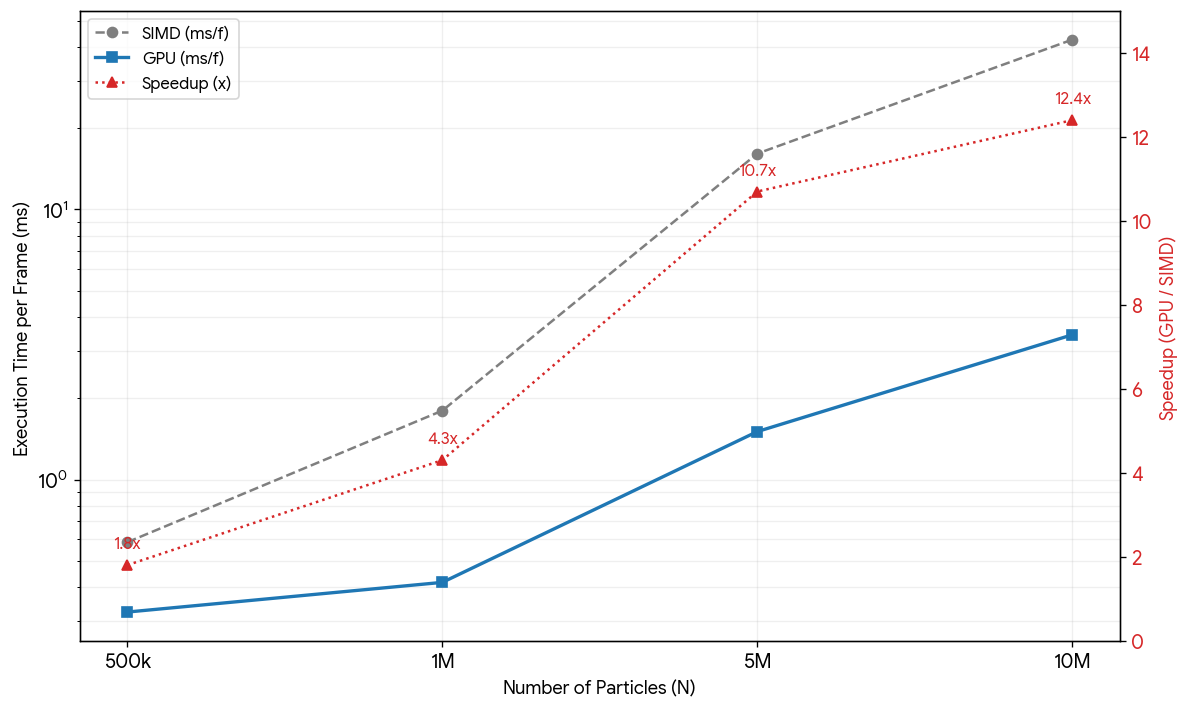
\includegraphics[width=0.9\columnwidth]{figures/GTX_scalingMS.png}}
  \caption{Scaling: ms SIMD CPU vs GTX960M.}
  \label{fig:GTX_scalingMS}
\end{figure}

As $N$ grows the GPU's parallel capture kernel and $O(N \cdot k)$ grid-based 
collision scale far better than the CPU's $O(N^2)$ brute-force, reaching a 
\textbf{12.4$\times$ speedup} at $N = 10^7$. \\
Overhead grows modestly with N and never exceeds 3\% of frame time at large scales, 
confirming that PCIe transfer cost is amortized at scale.

\subsection{Jetson Nano Per-Kernel Timing Physics Scenario}

These scenarios use a small number of particles ($N = 10^5$)
causing the simulation on GPU to remain in the fused regime.

\begin{table}[H]
  \caption{Wet snow. \\-}
  \label{tab:jetson_scenario1_timing}
  \centering
  \scriptsize
  \begin{tabular}{@{}lcccccc@{}}
    \toprule
    \textbf{Kernel} & \textbf{SISD (ms)} & \textbf{SIMD (ms)} & \textbf{GPU (ms)} \\
    \midrule
    captureFromSnowpack           & 0.2554 & 0.1949 & 0.0329 \\
    forceTether                   & 0.0354 & 0.0057 & 0.0000 \\
    shellGrid                     & 0.1062 & 0.0327 & 0.0000 \\
    bruteForceCollision           & 0.3813 & 0.0628 & 0.0000 \\
    integrateGround               & 0.0237 & 0.0057 & 0.0000 \\
    shellPhysicsFused             & 0.0000 & 0.0000 & 0.1246 \\
    coreUpdate                    & 0.0004 & 0.0003 & 0.0000 \\
    Overhead                      & 0.0012 & 0.0007 & 0.0192 \\
    \bottomrule
    FPS                           & 1244.3 & 3302.7 & 5660.1
  \end{tabular}
\end{table}

\begin{table}[H]
  \caption{Dry snow.\\--wetness-max 0.3 --stick-k1 3.0}
  \label{tab:jetson_scenario2_timing}
  \centering
  \scriptsize
  \begin{tabular}{@{}lccc@{}}
    \toprule
    \textbf{Kernel} & \textbf{SISD (ms)} & \textbf{SIMD (ms)} & \textbf{GPU (ms)} \\
    \midrule
    captureFromSnowpack           & 0.1497 & 0.1870 & 0.0468 \\
    forceTether                   & 0.0164 & 0.0061 & 0.0000 \\
    shellGrid                     & 0.0452 & 0.0222 & 0.0000 \\
    bruteForceCollision           & 0.1452 & 0.0248 & 0.0000 \\
    integrateGround               & 0.0112 & 0.0065 & 0.0000 \\
    shellPhysicsFused             & 0.0000 & 0.0000 & 0.1083 \\
    coreUpdate                    & 0.0004 & 0.0003 & 0.0000 \\
    Overhead                      & 0.0012 & 0.0006 & 0.0331 \\
    \bottomrule
    FPS                           & 2707.5 & 4039.0 & 5314.7
  \end{tabular}
\end{table}

\begin{table}[H]
  \caption{\centering Amplified avalanche feedback. \\ \centering --stick-rboost 10.0}
  \label{tab:jetson_scenario3_timing}
  \centering
  \scriptsize
  \begin{tabular}{@{}lccc@{}}
    \toprule
    \textbf{Kernel} & \textbf{SISD (ms)} & \textbf{SIMD (ms)} & \textbf{GPU (ms)} \\
    \midrule
    captureFromSnowpack           & 0.2489 & 0.2031 & 0.0498 \\
    forceTether                   & 0.0420 & 0.0076 & 0.0000 \\
    shellGrid                     & 0.1273 & 0.0389 & 0.0000 \\
    bruteForceCollision           & 0.4790 & 0.0719 & 0.0000 \\
    integrateGround               & 0.0285 & 0.0068 & 0.0000 \\
    shellPhysicsFused             & 0.0000 & 0.0000 & 0.1974 \\
    coreUpdate                    & 0.0004 & 0.0003 & 0.0000 \\
    Overhead                      & 0.0012 & 0.0007 & 0.0412 \\
    \bottomrule
    FPS                           & 1078.4 & 3036.5 & 3466.9
  \end{tabular}
\end{table}

\begin{table}[H]
  \caption{High inter-particle friction. \\ --part-friction 0.6}
  \label{tab:jetson_scenario4_timing}
  \centering
  \scriptsize
  \begin{tabular}{@{}lccc@{}}
    \toprule
    \textbf{Kernel} & \textbf{SISD (ms)} & \textbf{SIMD (ms)} & \textbf{GPU (ms)} \\
    \midrule
    captureFromSnowpack           & 0.2557 & 0.2188 & 0.0507 \\
    forceTether                   & 0.0351 & 0.0069 & 0.0000 \\
    shellGrid                     & 0.1067 & 0.0354 & 0.0000 \\
    bruteForceCollision           & 0.3818 & 0.0597 & 0.0000 \\
    integrateGround               & 0.0236 & 0.0068 & 0.0000 \\
    shellPhysicsFused             & 0.0000 & 0.0000 & 0.1723 \\
    coreUpdate                    & 0.0004 & 0.0003 & 0.0000 \\
    Overhead                      & 0.0012 & 0.0007 & 0.0363 \\
    \bottomrule
    FPS                           & 1242.9 & 3044.0 & 3854.4
  \end{tabular}
\end{table}

\begin{table}[H]
  \caption{Slope 45°.\\ --slope 45.0}
  \label{tab:jetson_scenario5_timing}
  \centering
  \scriptsize
  \begin{tabular}{@{}lccc@{}}
    \toprule
    \textbf{Kernel} & \textbf{SISD (ms)} & \textbf{SIMD (ms)} & \textbf{GPU (ms)} \\
    \midrule
    captureFromSnowpack           & 0.1840 & 0.1892 & 0.0447 \\
    forceTether                   & 0.0202 & 0.0066 & 0.0000 \\
    shellGrid                     & 0.0573 & 0.0247 & 0.0000 \\
    bruteForceCollision           & 0.1794 & 0.0287 & 0.0000 \\
    integrateGround               & 0.0138 & 0.0070 & 0.0000 \\
    shellPhysicsFused             & 0.0000 & 0.0000 & 0.1334 \\
    coreUpdate                    & 0.0004 & 0.0003 & 0.0000 \\
    Overhead                      & 0.0012 & 0.0007 & 0.0291 \\
    \bottomrule
    FPS                           & 2191.0 & 3890.7 & 4823.8
  \end{tabular}
\end{table}

\begin{figure}[H]
  \centering
  \includegraphics[width=\columnwidth]{figures/jetson_scenariocomparison.png}
  \caption{FPS comparison across the 5 physics scenarios on the Jetson Nano.}
  \label{fig:jetson_scenariocomparison}
\end{figure}

At $N = 10^5$, the Jetson Nano GPU slightly outperforms both CPU baselines in all five
physics scenarios---a stark contrast to the GTX\,960M, which is slower than
the CPU at this scale. The unified memory architecture eliminates PCIe transfer
overhead entirely, so even a single SM delivers a consistent GPU advantage;
kernel-launch and event overhead account for only 11--18\% of GPU frame time
vs.\ 35--50\% on the GTX\,960M.

\subsection{Scaling with Particle Count}

\begin{table}[H]
  \caption{$N = 500{,}000$.}
  \label{tab:jetson_scaling_500k}
  \centering
  \scriptsize
  \begin{tabular}{@{}lccc@{}}
    \toprule
    \textbf{Kernel} & \textbf{SIMD (ms)} & \textbf{GPU (ms)} \\
    \midrule
    captureFromSnowpack        & 1.5144 & 0.4723 \\
    forceTether                & 0.0311 & 0.0048 \\
    shellGrid                  & 0.2603 & 0.0198 \\
    neighborCollision          & 0.7858 & 0.1176 \\
    integrateGround            & 0.0249 & 0.0044 \\
    shellPhysicsFused          & 0.0000 & 0.3468 \\
    coreUpdate                 & 0.0004 & 0.0000 \\
    Overhead                   & 0.0010 & 0.6080 \\
    \bottomrule
    FPS                        & 382.0 & 635.4 \\
  \end{tabular}
\end{table}

\begin{table}[H]
  \caption{$N = 1{,}000{,}000$.}
  \label{tab:jetson_scaling_1m}
  \centering
  \scriptsize
  \begin{tabular}{@{}lcc@{}}
    \toprule
    \textbf{Kernel} & \textbf{SIMD (ms)} & \textbf{GPU (ms)} \\
    \midrule
    captureFromSnowpack        & 3.0397 & 0.6675 \\
    forceTether                & 0.0601 & 0.0158 \\
    shellGrid                  & 0.6560 & 0.1044 \\
    neighborCollision          & 2.5563 & 4.1633 \\
    integrateGround            & 0.0582 & 0.0127 \\
    shellPhysicsFused          & 0.0000 & 0.2029 \\
    coreUpdate                 & 0.0005 & 0.0000 \\
    Overhead                   & 0.0012 & 0.9778 \\
    \bottomrule
    FPS                        & 156.9 & 162.8 \\
  \end{tabular}
\end{table}

\begin{table}[H]
  \caption{$N = 5{,}000{,}000$.}
  \label{tab:jetson_scaling_5m}
  \centering
  \scriptsize
  \begin{tabular}{@{}lcc@{}}
    \toprule
    \textbf{Kernel} & \textbf{SIMD (ms)} & \textbf{GPU (ms)} \\
    \midrule
    captureFromSnowpack        &  14.9198 &   0.7978 \\
    forceTether                &   0.3281 &   0.0897 \\
    shellGrid                  &   4.7699 &   0.5537 \\
    neighborCollision          &  36.9670 & 174.8856 \\
    integrateGround            &   0.3268 &   0.0943 \\
    shellPhysicsFused          &   0.0000 &   0.0774 \\
    coreUpdate                 &   0.0005 &   0.0000 \\
    Overhead                   &   0.0016 &   1.4548 \\
    \bottomrule
    FPS                        & 17.4 & 5.6 \\
  \end{tabular}
\end{table}

N = 10M scaling was not possible due to GPU out-of-memory errors and a catastrophic performance drop on both CPU and GPU.\\[1em]

\begin{table}[H]
  \caption{GPU vs.\ SIMD CPU scaling with size $N$.}
  \label{tab:jetson_scaling}
  \centering
  \scriptsize
  \begin{tabular}{@{}rccccc@{}}
    \toprule
    \textbf{N} & \textbf{SIMD (FPS)} & \textbf{GPU (FPS)} & \textbf{SIMD (ms/f)} & \textbf{GPU (ms/f)} & \textbf{Speedup} \\
    \midrule
       500{,}000 &   382.0 &   635.4 &  2.618 &   1.574 & 1.7$\times$ \\
     1{,}000{,}000 &   156.9 &   162.8 &  6.372 &   6.144 & 1.0$\times$ \\
     5{,}000{,}000 &    17.4 &     5.6 & 57.314 & 177.953 & 0.3$\times$ \\
    10{,}000{,}000 &     -  &     -  &    -  &     -  &    -  \\
    \bottomrule
  \end{tabular}
\end{table}

\begin{figure}[H]
  \centering
  \fbox{\includegraphics[width=0.9\columnwidth]{figures/jetson_scalingFPS.png}}
  \caption{Scaling: FPS SIMD CPU vs Jetson Nano.}
  \label{fig:jetson_scalingFPS}
\end{figure}

\begin{figure}[H]
  \centering
  \fbox{\includegraphics[width=0.9\columnwidth]{figures/jetson_scalingMS.png}}
  \caption{Scaling: ms SIMD CPU vs Jetson Nano.}
  \label{fig:jetson_scalingMS}
\end{figure}

The Jetson Nano's single Maxwell SM (128 cores, 2048 max threads) is the
fundamental bottleneck at large $N$. With $\sim$72K shell particles and a
single SM limited to 2\,048 concurrent threads, the collision kernel
serialises into $\sim$36 sequential warp waves, each performing $O(k)$
neighbour lookups. This causes super-linear growth in execution time: the
shell grows only 6.7$\times$ from $N=10^6$ to $N=5{\times}10^6$, yet GPU
collision time grows 42$\times$ (4.16\,ms $\to$ 174.9\,ms), while the
4-core SIMD CPU grows only 14.5$\times$ on the same workload.\\
In contrast, the 4-core multi-threaded SIMD CPU scales far more gracefully 
under the same workload.\\ A multi-SM desktop GPU—such as the GTX 960M with 
5 SMs and 640 cores effectively mitigates this bottleneck by distributing 
the massive wave volume across multiple physical processing blocks, 
maintaining high throughput even in heavily saturated particle regimes.
% !TEX root = ../paper.tex
\section{Conclusion}
\label{sec:conclusion}

We presented a GPU-accelerated Discrete Element Method simulation of a
growing snowball rolling down an inclined slope, targeting NVIDIA Maxwell
hardware (GTX~960M and Jetson~Nano). The key takeaways are:

\begin{enumerate}
  \item \textbf{Architecture-aware optimisation matters.} On resource-constrained
        Maxwell GPUs, each register, each kilobyte of shared memory, and each
        kernel launch has measurable impact. The warp-cooperative tiling design,
        zero-spill register allocation, and gated event recording are all
        responses to specific Maxwell bottlenecks (no hardware FP32 atomics,
        48\,KB shared memory limit, high per-command driver overhead).

  \item \textbf{Adaptive fusion pays off.} The dual-path pipeline
        (mega-fused for $N \leq 2048$, grid-based for $N > 2048$) eliminates
        launch overhead during the initial growth phase while seamlessly
        transitioning to the scalable $O(N \cdot k)$ path as the particle
        count increases.

  \item \textbf{Zero spill trumps 100\% occupancy.} Accepting 62.5--75\%
        occupancy in exchange for keeping all variables in physical registers
        avoids DRAM-backed spill costs ($\sim$300 cycles per access) and
        yields better real-world performance than forcing higher occupancy
        through aggressive register limiting.

  \end{enumerate}

\subsection{Future Work}

Several extensions could be developed:

\begin{itemize}
  \item \textbf{Multi-GPU / domain decomposition}: partitioning the spatial
        grid across multiple GPUs via halo exchange for simulations with 
        very large shell particle counts (refer to Attachment 1).
  \item \textbf{Persistent-contact DEM}: tracking tangential spring history
        across frames for more accurate friction modelling, at the cost of
        additional per-pair state.
  \item \textbf{Volta+ optimisations}: on SM~7.0+, hardware
        \texttt{atomicAdd(float)} eliminates CAS loops, potentially making
        symmetric collision viable again; cooperative groups could replace
        warp-level synchronisation.
  \item \textbf{3D terrain}: replacing the infinite plane with a height-map
        or mesh-based terrain for realistic mountain geometry.
\end{itemize}


\section*{Project Code}
The complete source code for \textbf{Angry Santa} is available on GitHub: \url{https://github.com/politos336145/GPU-Programming-2025-2026}

\section*{Acknowledgments}
The authors thank the GPU Programming course staff at Politecnico di Torino for guidance and access to the Jetson Nano development kits.

\nocite{cuda_programming_guide,cuda_best_practices,cuda_toolkit,nsight_tools,cub_library,vulkan_api,dear_imgui}

\bibliographystyle{IEEEtran}
\bibliography{refs}

\end{document}
